\documentclass[12pt]{extarticle}
\usepackage{tikz}
\usetikzlibrary{calc}
\usepackage{eso-pic}
\usepackage{datetime}
\usepackage{lipsum}
\usepackage{graphicx}
\graphicspath{/home/pratik/Desktop/}
\AddToShipoutPictureBG{%
\begin{tikzpicture}[overlay,remember picture]
\draw[line width=6pt]
    ($ (current page.north west) + (0.8cm,-0.8cm) $)
    rectangle
    ($ (current page.south east) + (-0.8cm,0.8cm) $);
\draw[line width=1.5pt]
    ($ (current page.north west) + (1.2cm,-1.2cm) $)
    rectangle
    ($ (current page.south east) + (-1.2cm,1.2cm) $);
\end{tikzpicture}
}
\usepackage{color}
\date{}
\author{\textbf{Vaibhav Vashisht} 2016CSJ0002  \\\textbf{Pratik Parmar} 2016CSJ0049}
\title{\textbf{COP290: Design Practices\\ Design Document \\ AC Circuit Solver  }}
\begin{document}
\maketitle
\newpage
\tableofcontents
\newpage
\section{Introduction}

\subsection{Purpose}
The purpose of this document is to describe the implementation of AC Circuit Solver application developed by us.
\subsection{Scope}
The software consists of two major function.First to render the ac circuit as an SVG image and second is to solve the circuit correclty.
\subsection{Definitions}
\begin{enumerate}
\item \textbf{Netlist:} A netlist is a textual description of a circuit made of components. Components are generally gates, so generally a Netlist is a connection. of gates. A netlist can also be a connection of resistors, capacitors or. transistors, which is a netlist when used in analog simulation tools. 
\item \textbf{Parsing: }A parser is a compiler or interpreter component that breaks data into smaller elements for easy translation into another language and the process of doing this is called Parsing. 
\end{enumerate}
\section{Overall Design}
In this project we are given an input file which contains the netlist describing the circuit.For reading and checking the strings
from the input file we have used lex to get tokens then check whether they match the given format.
\subsection{Components}
\begin{enumerate}
\item \textbf{Component Class:}
The class \textbf{Component} consists 
Component(Resistor, Capacitor, Inductor) information:
\begin{enumerate}
\item \textbf{Type:} Whether the component is resistor or capacitor or inductor
Nets b/w which component is connected.
\item \textbf{Magnitude: } Resistance/Capacitance/ Inductance depending upon the 
type of the component.
\item \textbf{Index:} Returns the index of the component i.e if resistor name is r1 then it returns 1.
\item \textbf{Initial Net and Final Net: } Stores value of Nets between which Component is located. 
\end{enumerate} 
\item \textbf{Source Class:}
This class consists Sources(Current/Voltage source) information
\begin{enumerate}
\item \textbf{Type: }Whether source is a Voltage source or a Current source.
\item \textbf{Index: }Stores the id of Source.
\item \textbf{Initial and Final Net: }Stores values of Nets between which Source is located.
\item \textbf{DCO: }Stores Value of DCO of the Source.
\item \textbf{Amplitude: }Stores value of Amplitude of the Source.
\item \textbf{Frequency: }Stores Frequency of the Source.
\item \textbf{Delay: }Stores magnitude of Delay in second for the Source.
\item \textbf{Damping Factor: }Stores value of Damping factor for the Source.
\end{enumerate}

\end{enumerate}

\subsection{SVG Rendering}
\paragraph{Drawing Nets}
All the components are traversed to check the nets b/w which that component is drawn.As we get new nets we mark them on the screen and mantain a boolean array to ensure the nets which have already been marked need not to be marked again.  

\paragraph{Drawing Components}
The data collected from both the classes is used to construct the circuit described by the netlist.SVG code has been written for drawing each component separately and using data from both the classes we can arrange the componenets accordingly to get the desired circuit.For eg to draw a resistor b/w two nets strps followed are as follows-:
First we traverse among the componenets and detect whether the component is resistor or capacitor so on.Once we detect that the component is a resistor we check b/w which nets we need to draw the component.Send the co-ordinates of the nets found as an input to DrawResistor function.And this function draws the resisitor b/w the given nets.
\\
\begin{center}
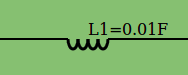
\includegraphics[width=6.5cm, height=3cm]{Inductor}
\hspace{2mm}
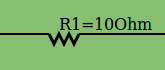
\includegraphics[width=6.5cm, height=3cm]{Resistor}
\end{center}
\paragraph{Drawing Sources}
Sources are drawn in the same way as components,only difference is that we have to mantain some more variables such as DC offset,frequency for sources which has been handled in Sources class.  
\\
\begin{center}
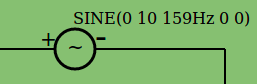
\includegraphics[width=6.5cm, height=3cm]{Source}
\end{center}

\paragraph{Overlapping Components}
To prevent overlappong components we mantain a count of no. of components already drawn b/w the nets and the new component is drawn farther from already drawn components so that circuit looks neat and components are far away from each other. 

\paragraph{Displaying net,component number and type}
At the time of drawing the component/net their name and value if any is drawn simultaneously according to the co-ordinates of the component.

\paragraph{Scaling}
As the number of nets increase distance b/w consecutive nets decreases to accomodate more number of nets,also the size of the allocated screen also increases to allow more number of nets to be displayed.Zooming may be required to view the circuit clearly if number of nets is very large. 

\paragraph{How is SVG Code generated?}
Actually all the drawing functions such as DrawResistor()/DrawCap() etc output SVG Code into a html file which further can be rendered in browser.
\begin{center}
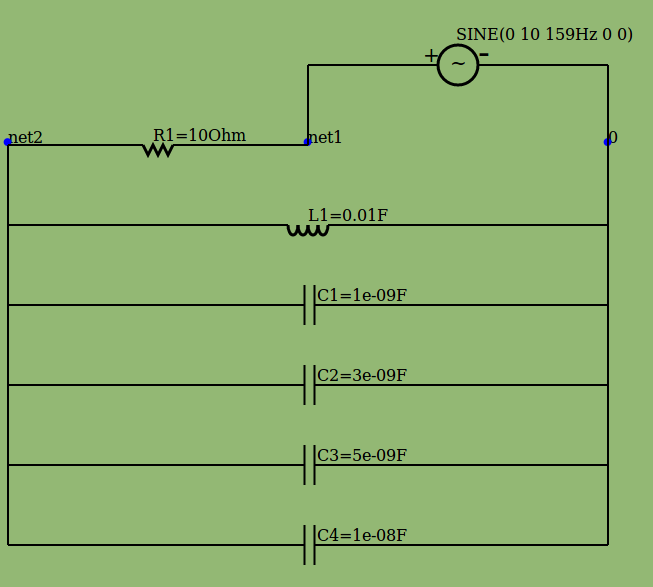
\includegraphics[width=14cm, height=8cm]{Top}
\end{center}
\section{Circuit Solving}

Any ac circuit can be simplified to a circuit of form given below which consists of only two components,Net Volatge/Current Source and Net Impeadence of the circuit which can be solved using phasor analysis.
\subsection{Impedence RLC Series}
\begin{enumerate}
\item RL-Series Combination$$Z_{RL-series}=\sqrt{R^{2}+X{_{L}}{^{2}}} $$
\item RC-Series Combination$$Z_{RC-series}=\sqrt{R^{2}+X{_{C}}{^{2}}} $$
\item LC-Series Combination$$Z_{LC-series}=\sqrt{{(X_{L}-X{_{C})}}{^{2}}} $$
\item RLC-Series Combination$$Z_{RLC-series}=\sqrt{R^{2}+{(X_{L}-X{_{C})}}{^{2}}} $$
\item Inductive Reactance $$X_{L}=2\pi fL$$
\item Capacitive Reactance $$X_{C}=\frac{1}{2\pi fC}$$
\end{enumerate}
\subsection{Impedence RLC Parallel}
\begin{enumerate}
\item RL-Parallel Combination$$\frac{1}{Z_{RL-parallel}}=\sqrt{\left(\frac{1}{R}\right)^{2}+\left(\frac{1}{X_{L}}\right)^{2}} $$
\item RC-Parallel Combination$$\frac{1}{Z_{RC-parallel}}=\sqrt{\left(\frac{1}{R}\right)^{2}+\left(\frac{1}{X_{C}}\right)^{2}} $$
\item LC-Parallel Combination$$\frac{1}{Z_{LC-parallel}}=\sqrt{\left({{\frac{1}{X_{L}}}-{\frac{1}{X_{C}}}}\right)^{2}} $$
\item RLC-Parallel Combination$$\frac{1}{Z_{RLC-parallel}}=\sqrt{{\left({\frac{1}{R}}^{2}\right)}+\left({{\frac{1}{X_{L}}}-{\frac{1}{X_{C}}}}\right)^{2}} $$
\item Inductive Reactance $$X_{L}=2\pi fL$$
\item Capacitive Reactance $$X_{C}=\frac{1}{2\pi fC}$$
\end{enumerate}
\paragraph{Solution}
Using Formulae for Impedence we will simplify the circuit to get overall Impedence of the circuit$$Z_{net}$$ As we already know the Voltage of the Circuit then using the formula given below we can find the Current in the circuit.
$$I=\frac{V}{Z_{net}}$$
\section{Testing}

\subsection{Circuit Testing} We will check for some test cases that circuit drawn by the application corresponds to that given in the netlist.We will also check for some corner cases for eg circuit with large no. of nets etc
\subsection{Parameters Testing}We will check whether voltage and current values for some circuits match with what is expected for that circuit.
\section{Software Requirement}
Following Software/Packages are Required for running this application.
\begin{enumerate}
\item Linux Based Operating System preferably Ubuntu
\item GNU g++ Compiler for C++\\
For Compilation of C++ program
\item Flex(Fast Lexical Analyser Generator)\\
It is Used to Generate Scanner for Netlist file so as to allow only useful lexemes as a input and Generates tokens as output.
\item Bison\\
It is Used to Defined a Grammar for Netlist Syntax so that we can handle any syntactical error occuring in the input.
\item HTML Viewer or Web Browser(Firefox or Chrome)\\
It is Used as an image viewer for SVG file. As web browsers allow Javascript that can be used to make image more interactive for the user.
\end{enumerate}

\section{Technical Process}
Following would be the Languages/tools would be used to develop this application
\begin{enumerate}
\item Functionality: C++\\
	Parsing of the  Netlist file , generation of SVG image for AC circuit and Solving the AC circuit is to be done in C++.
\item Image Rendering: SVG\\
Scalable Vector Graphics are used for generating of AC circuit's image.
\item Interactivity in Image: JavaScript\\
Adding Functionallity in Image is done using Javascript. It will be used to provide interactivity in the image as if you click on any component of the circuit,voltage across that component and more information we be displayed. Also it will provide Zooming facility to the image.
\item Styling: CSS\\
To make the page containing the SVG image looks stylish.
\item Layout: HTML and XML\\
For Designing the page containing SVG image.
\item Scripting: Bash\\
It is used in the makefile.
\end{enumerate}
\end{document}

